\chapter{Thermo-optical topology optimization problems}
%CHECK COPYRIGHT FOR FIGURES AND REPRINTS
%In this chapter we will focus on the effects of multiphysics couplings in nanophotonic devices, reviewing state-of-the-art research, 
%highlighting open topology optimization problems, and presenting our contributions to the field.
%We will focus on three main classes of multiphysics couplings: thermo-optical, opto-mechanical, and electro-optical systems.
%\begin{figure}[tb]
%    \centering
%    \makebox[\textwidth][c]{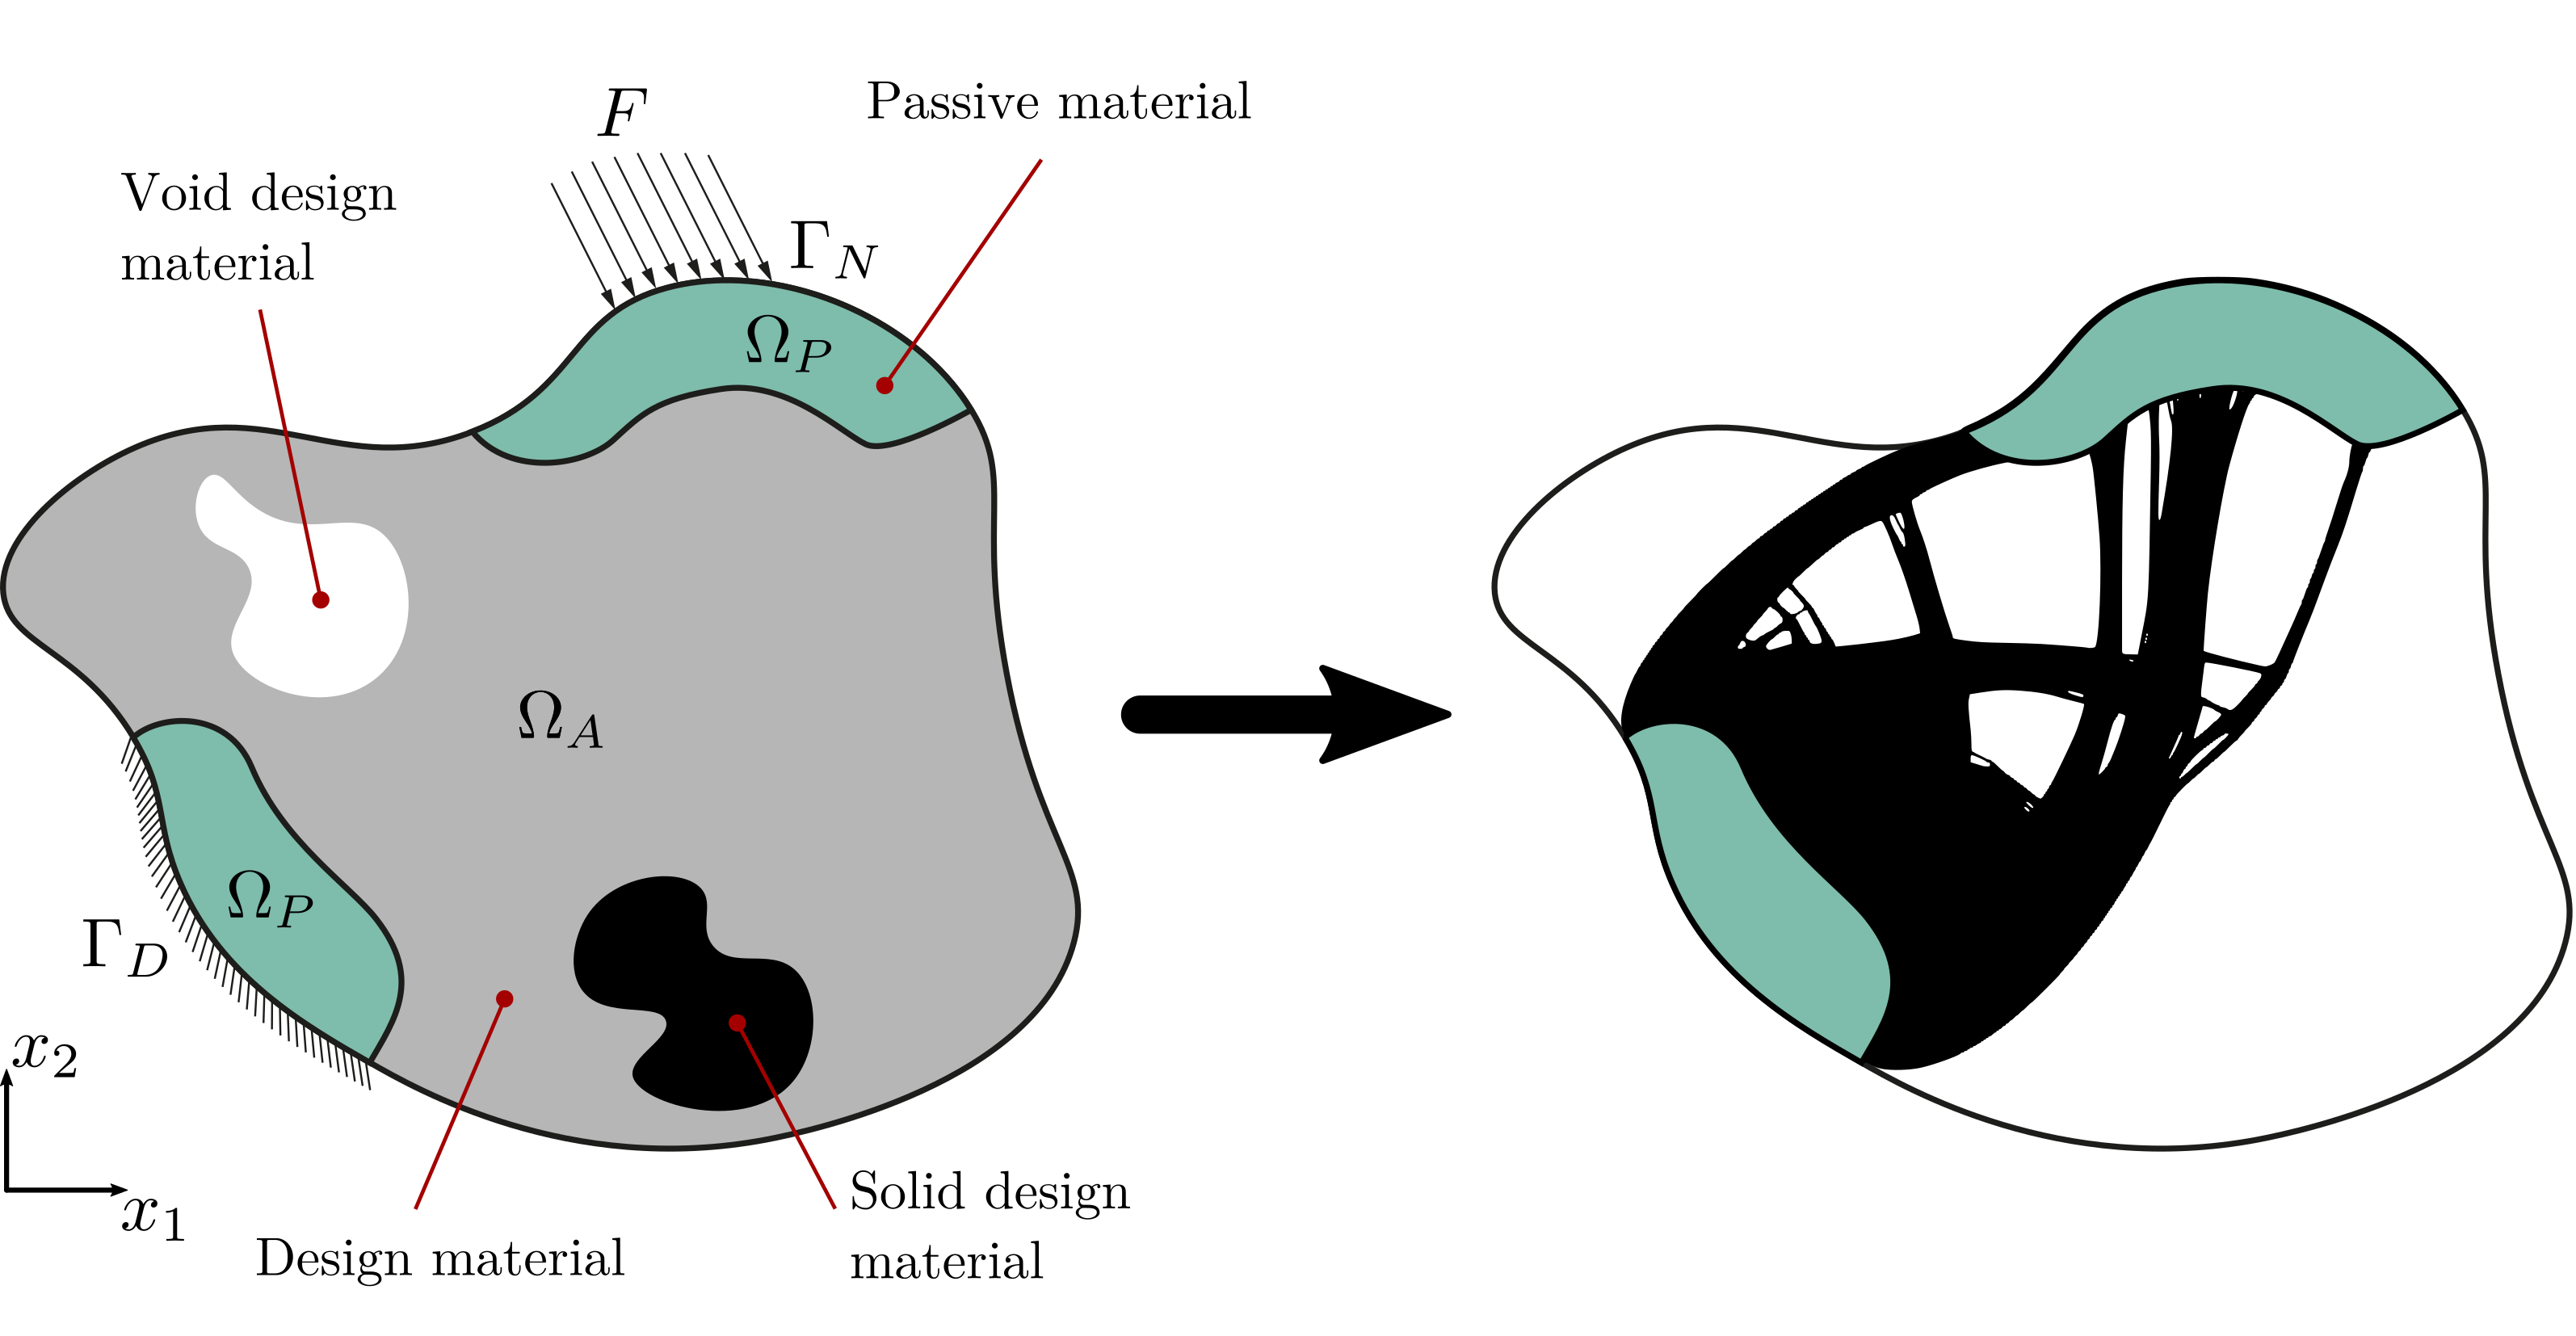
\includegraphics[width=1\imwidth]{figures/simpModel.png}}%
%    \caption{Bla bla bla...}
%    \label{fig:illustateTopOpt}
%\end{figure
%\begin{equation}
%    (EIu'')'' = q
%\end{equation}
%\beginfigure}[tb]
%    \centering
%    \makebox[\textwidth][c]{\begin{tikzpicture}[remember picture]
    \begin{scope}[xshift=0mm]
        % angle (deg)
        \newcommand\ai{10}
        % line width
        \newcommand\wi{1pt}
        % cell size
        \newcommand\cellsize{3}
        % Rank-$N$ size
        \newcommand\di{0.75}

        % cell
        \draw[gray!10,   fill=gray!10, rotate around={\ai:(0,0)}] (0,0) rectangle (\cellsize,\cellsize) node (rect1) {};
        \draw[black!60, fill=black!60, rotate around={\ai:(0,0)}] (0,0) rectangle (\di,\cellsize);

        % orientation frame
        \draw[black, -stealth, line width=\wi, rotate around={\ai:({\di*cos(\ai) - \cellsize/2*sin(\ai)},{\di*sin(\ai) + \cellsize/2*cos(\ai)})}] ({\di*cos(\ai) - \cellsize/2*sin(\ai)},{\di*sin(\ai) + \cellsize/2*cos(\ai)}) -- ({\di*cos(\ai) - \cellsize/2*sin(\ai) + 0.75},{\di*sin(\ai) + \cellsize/2*cos(\ai)});
        \draw[black, -stealth, line width=\wi, rotate around={\ai:({\di*cos(\ai) - \cellsize/2*sin(\ai)},{\di*sin(\ai) + \cellsize/2*cos(\ai)})}] ({\di*cos(\ai) - \cellsize/2*sin(\ai)},{\di*sin(\ai) + \cellsize/2*cos(\ai)}) -- ({\di*cos(\ai) - \cellsize/2*sin(\ai)},{\di*sin(\ai) + \cellsize/2*cos(\ai) + 0.75});

        % local frame
        \draw[black, -stealth, dashed, line width=\wi] (0,0) -- ({\cellsize + 0.8},0);
        \draw[black, -stealth, dashed, line width=\wi] (0,0) -- (0,{\cellsize + 0.8});

        % ruler
        \draw[black, |-|, line width=\wi, rotate around={\ai:(0,0)}] (0,0) -- (\cellsize,0);
        \draw[black,  -|, line width=\wi, rotate around={\ai:(0,0)}] (0,0) -- (\di,0);

        % arc
        \draw[black, dotted, line width=\wi] (\cellsize,0) arc (0:\ai:\cellsize);

        % annotation
        \draw (\cellsize + 0.7, -0.3) node {$x_1 / \epsilon^3$};
        \draw (-0.5, \cellsize + 0.8) node {$x_2 / \epsilon^3$};
        \draw (\cellsize/2,-0.75) node {Rank-$1$};

        \draw[rotate around={{\ai/2}:(0,0)}] ({\cellsize+0.3},0) node {$\theta_1$};

        \draw[rotate around={{\ai}:(0,0)}] ({\di/2},0.4) node [rotate around={{\ai}:(0,0)}] {$\mu_1$};
        \draw[rotate around={{\ai}:(0,0)}] ({(\cellsize - \di)/2 + \di},0.4) node [rotate around={{\ai}:(0,0)}] {$1-\mu_1$};

        \draw[rotate around={{\ai}:(0,0)}] ({0+0.4},{\cellsize-0.4}) node [rotate around={{\ai}:(0,0)}] {$(+)$};
        \draw[rotate around={{\ai}:(0,0)}] ({\cellsize-0.4},{\cellsize-0.4}) node [rotate around={{\ai}:(0,0)}] {$(-)$};
        \coordinate (A) at (rect1.north);


        \draw[rotate around={\ai:({\di*cos(\ai) - \cellsize/2*sin(\ai)},{\di*sin(\ai) + \cellsize/2*cos(\ai)})}] ({\di*cos(\ai) - \cellsize/2*sin(\ai)+1} , {\di*sin(\ai) + \cellsize/2*cos(\ai) + 0.2}) node {$\mathbf{n}_1$};
        \draw[rotate around={\ai:({\di*cos(\ai) - \cellsize/2*sin(\ai)},{\di*sin(\ai) + \cellsize/2*cos(\ai)})}] ({\di*cos(\ai) - \cellsize/2*sin(\ai) + 0.3} , {\di*sin(\ai) + \cellsize/2*cos(\ai) + 1}) node {$\mathbf{m}_1$};



    \end{scope}
    \begin{scope}[xshift=45mm]
        % angle (deg)
        \newcommand\ai{15}
        % line width
        \newcommand\wi{1pt}
        % cell size
        \newcommand\cellsize{3}
        % Rank-$N$ size
        \newcommand\di{0.6}

        % cell
        \draw[gray!40,   fill=gray!40, rotate around={\ai:(0,0)}] (0,0) rectangle (\cellsize,\cellsize) node (rect2) {};
        \draw[black!60, fill=black!60, rotate around={\ai:(0,0)}] (0,0) rectangle (\di,\cellsize);

        % orientation frame
        \draw[black, -stealth, line width=\wi, rotate around={\ai:({\di*cos(\ai) - \cellsize/2*sin(\ai)},{\di*sin(\ai) + \cellsize/2*cos(\ai)})}] ({\di*cos(\ai) - \cellsize/2*sin(\ai)},{\di*sin(\ai) + \cellsize/2*cos(\ai)}) -- ({\di*cos(\ai) - \cellsize/2*sin(\ai) + 0.75},{\di*sin(\ai) + \cellsize/2*cos(\ai)});
        \draw[black, -stealth, line width=\wi, rotate around={\ai:({\di*cos(\ai) - \cellsize/2*sin(\ai)},{\di*sin(\ai) + \cellsize/2*cos(\ai)})}] ({\di*cos(\ai) - \cellsize/2*sin(\ai)},{\di*sin(\ai) + \cellsize/2*cos(\ai)}) -- ({\di*cos(\ai) - \cellsize/2*sin(\ai)},{\di*sin(\ai) + \cellsize/2*cos(\ai) + 0.75});

        % local frame
        \draw[black, -stealth, dashed, line width=\wi] (0,0) -- ({\cellsize + 0.8},0);
        \draw[black, -stealth, dashed, line width=\wi] (0,0) -- (0,{\cellsize + 0.8});

        % ruler
        \draw[black, |-|, line width=\wi, rotate around={\ai:(0,0)}] (0,0) -- (\cellsize,0);
        \draw[black,  -|, line width=\wi, rotate around={\ai:(0,0)}] (0,0) -- (\di,0);

        % arc
        \draw[black, dotted, line width=\wi] (\cellsize,0) arc (0:\ai:\cellsize);

        % annotation
        \draw (\cellsize + 0.7, -0.3) node {$x_1 / \epsilon^2$};
        \draw (-0.5, \cellsize + 0.8) node {$x_2 / \epsilon^2$};
        \draw (\cellsize/2,-0.75) node {Rank-$2$};

        \draw[rotate around={{\ai/2}:(0,0)}] ({\cellsize+0.3},0) node {$\theta_2 + \pi/4$};

        \draw[rotate around={{\ai}:(0,0)}] ({\di/2},0.4) node [rotate around={{\ai}:(0,0)}] {$\mu_2$};
        \draw[rotate around={{\ai}:(0,0)}] ({(\cellsize - \di)/2 + \di},0.4) node [rotate around={{\ai}:(0,0)}] {$1-\mu_2$};

        \draw[rotate around={{\ai}:(0,0)}] ({0+0.4},{\cellsize-0.4}) node [rotate around={{\ai}:(0,0)}] {$(+)$};
        \draw[rotate around={{\ai}:(0,0)}] ({\cellsize-0.9},{\cellsize-0.4}) node [rotate around={{\ai}:(0,0)}] (B) {$(\text{Rank-1})$};
        \coordinate (B2) at (rect2.north);


        \draw[rotate around={\ai:({\di*cos(\ai) - \cellsize/2*sin(\ai)},{\di*sin(\ai) + \cellsize/2*cos(\ai)})}] ({\di*cos(\ai) - \cellsize/2*sin(\ai)+1} , {\di*sin(\ai) + \cellsize/2*cos(\ai) + 0.2}) node {$\mathbf{n}_2$};
        \draw[rotate around={\ai:({\di*cos(\ai) - \cellsize/2*sin(\ai)},{\di*sin(\ai) + \cellsize/2*cos(\ai)})}] ({\di*cos(\ai) - \cellsize/2*sin(\ai) + 0.3} , {\di*sin(\ai) + \cellsize/2*cos(\ai) + 1}) node {$\mathbf{m}_2$};


    \end{scope}
    \begin{scope}[xshift=90mm]
        % angle (deg)
        \newcommand\ai{20}
        % line width
        \newcommand\wi{1pt}
        % cell size
        \newcommand\cellsize{3}
        % Rank-$N$ size
        \newcommand\di{1.0}

        % cell
        \draw[gray!60,   fill=gray!60, rotate around={\ai:(0,0)}] (0,0) rectangle (\cellsize,\cellsize);
        \draw[black!60, fill=black!60, rotate around={\ai:(0,0)}] (0,0) rectangle (\di,\cellsize);

        % orientation frame
        \draw[black, -stealth, line width=\wi, rotate around={\ai:({\di*cos(\ai) - \cellsize/2*sin(\ai)},{\di*sin(\ai) + \cellsize/2*cos(\ai)})}] ({\di*cos(\ai) - \cellsize/2*sin(\ai)},{\di*sin(\ai) + \cellsize/2*cos(\ai)}) -- ({\di*cos(\ai) - \cellsize/2*sin(\ai) + 0.75},{\di*sin(\ai) + \cellsize/2*cos(\ai)});
        \draw[black, -stealth, line width=\wi, rotate around={\ai:({\di*cos(\ai) - \cellsize/2*sin(\ai)},{\di*sin(\ai) + \cellsize/2*cos(\ai)})}] ({\di*cos(\ai) - \cellsize/2*sin(\ai)},{\di*sin(\ai) + \cellsize/2*cos(\ai)}) -- ({\di*cos(\ai) - \cellsize/2*sin(\ai)},{\di*sin(\ai) + \cellsize/2*cos(\ai) + 0.75});

        % local frame
        \draw[black, -stealth, dashed, line width=\wi] (0,0) -- ({\cellsize + 0.8},0);
        \draw[black, -stealth, dashed, line width=\wi] (0,0) -- (0,{\cellsize + 0.8});

        % ruler
        \draw[black, |-|, line width=\wi, rotate around={\ai:(0,0)}] (0,0) -- (\cellsize,0);
        \draw[black,  -|, line width=\wi, rotate around={\ai:(0,0)}] (0,0) -- (\di,0);

        % arc
        \draw[black, dotted, line width=\wi] (\cellsize,0) arc (0:\ai:\cellsize);

        % annotation
        \draw (\cellsize + 0.7, -0.3) node {$x_1 / \epsilon$};
        \draw (-0.5, \cellsize + 0.8) node {$x_2 / \epsilon$};
        \draw (\cellsize/2,-0.75) node {Rank-$3$};

        \draw[rotate around={{\ai/2}:(0,0)}] ({\cellsize+0.3},0) node {$\theta_3 - \pi/2$};

        \draw[rotate around={{\ai}:(0,0)}] ({\di/2},0.4) node [rotate around={{\ai}:(0,0)}] {$\mu_3$};
        \draw[rotate around={{\ai}:(0,0)}] ({(\cellsize - \di)/2 + \di},0.4) node [rotate around={{\ai}:(0,0)}] {$1-\mu_3$};

        \draw[rotate around={{\ai}:(0,0)}] ({0+0.4},{\cellsize-0.4}) node [rotate around={{\ai}:(0,0)}] {$(+)$};
        \draw[rotate around={{\ai}:(0,0)}] ({\cellsize-0.9},{\cellsize-0.4}) node [rotate around={{\ai}:(0,0)}] (C) {$(\text{Rank-2})$};


        \draw[rotate around={\ai:({\di*cos(\ai) - \cellsize/2*sin(\ai)},{\di*sin(\ai) + \cellsize/2*cos(\ai)})}] ({\di*cos(\ai) - \cellsize/2*sin(\ai)+1} , {\di*sin(\ai) + \cellsize/2*cos(\ai) + 0.2}) node {$\mathbf{n}_3$};
        \draw[rotate around={\ai:({\di*cos(\ai) - \cellsize/2*sin(\ai)},{\di*sin(\ai) + \cellsize/2*cos(\ai)})}] ({\di*cos(\ai) - \cellsize/2*sin(\ai) + 0.3} , {\di*sin(\ai) + \cellsize/2*cos(\ai) + 1}) node {$\mathbf{m}_3$};

    \end{scope}
    \path[-latex,black,thick] (A) edge [bend left=50] (B);
    \path[-latex,black,thick] (B2) edge [bend left=50] (C);
\end{tikzpicture}}%
%    \caption{Bla bla bla...}
%    \label{fig:Rank}
%\end{figure}
%\section{Coupled optical systems}
%TODO: Include if we end up doing the Green's function study.
% Make a connection to the Green's function formalism and derive system of coupled equations.
%\section{Thermo-optical systems~\cite{ownpub0}}\label{sec:thermo_optical}
Thermo-optical systems exploit the interplay between the temperature and electromagnetic fields to enable active control over optical properties. 
The main mechanism behind this coupling is the thermo-optic effect, 
in which the refractive index of a material changes as a function of temperature. 
This effect plays a central role in many integrated photonics application; such as,
 optical phase shifters~\cite{TOPS_1, TOPS_2, TOPS_3}, reconfigurable photonic circuits~\cite{program, PIC}, and thermally tunable switches~\cite{switch, switch_2} and filters~\cite{filter}.

 Despite its wide usage, optimizing thermo-optical devices remains challenging due to the intricate coupling 
 between thermal and optical physics. Topology optimization offers a systematic design optimization solution, with application examples in
  thermo-optical phase shifters~\cite{TOPS_heat, ownpub0}, optical mirror-like thermo-mechanical structures~\cite{opt_perf}, and
strcutural integrity constraints~\cite{structural_heat}, among others.

In the following sections, we summarize how to model and optimize thermo-optic systems, 
with special focus on our research contribution~\cite{ownpub0}, which to the best of our knowledge,
extends the state-of-the art uncoupled and single-physics thermo-optic topology optimization frameworks by, for the first time, considering 
the coupled physical problem.

\section{The thermo-optic effect}

To model the coupled thermo-optical topology optimization problem, we combine the governing equation of the optical model [\eqref{eq:wave_eq}]
with a heat transfer model. The simplest heat trasfer model is the steady-state heat equation, which describes the
heat transfer in a medium due to conduction and heat sources. The heat equation is given by
\begin{equation}\label{eq:heat}
    -\nabla \cdot (\kappa \nabla T) = Q
\end{equation}
where $T$ is the temperature, $\kappa$ is the thermal conductivity, and $Q$ is a volumetric heat source. Note that this equation can be
extended by consider convection and radiation effects, which may be important in some thermo-optical systems (see the boundary conditions
in~\cite{ownpub0}).

This temperature can be coupled to the optical response via the therm-optic coefficient (TOC), which links the temperature field
with the refractive index of the material, typically approximated with the linear relation\footnote{Large temperature gradients may lead to nonlinear effects, requiring higher order terms.}
\begin{equation}
n(\mathbf{r}) = n_0 + \text{TOC} \cdot \left[T(\mathbf{r}) - T_0\right],
\end{equation}
where $n_0$ and $T_0$ are the reference (unheated) refractive index and reference temperature, respectively. Thus, to solve a problem coupled throught the TOC, one first solves the heat equation
to determine the temperature, which can be used to determine
the spatially varying refractive index, which is then used in \eqref{eq:wave_eq} to determine the optical field. In topology optimization
problems, one uses an additional material interpolation to link the physical field with the design-dependent conductivity, or heat source.

\section{Thermo-optical phase-shifter topology optimization~\cite{ownpub0}}

Among the many applications that utilize the thermo-optic coefficient, we find integrated photonic circuit components, which rely on the large 
TOC of silicon ($\text{TOC} \approx 1.8 \cdot 10^{-4}\, \text{K}^{-1}$) at room-temperature ($\approx300$ K) and telecom wavelength 
($\lambda=1.55$ \textmu m)~\cite{thermo-optic-coef}. One of those components is the thermo-optical phase shifter, which, as shown in \figref{fig:thermo_opt},
uses a heating device to locally modify the refractive index of a waveguide structure to induce a phase shift ($\Delta \Phi$) in the propagating optical mode
\begin{equation*}
\Delta \Phi = \frac{2\pi L}{\lambda} \Delta n_\text{eff},
\end{equation*}
where $L$ is the device length and $\Delta n_\text{eff} = n_\text{eff, heated} - n_\text{eff, unheated}$ is the change of the effective index of the waveguide. 

\subsection*{The effective index via waveguide finite-element analysis}

In order to calculate the phase-shift one thus needs to find the effective index of an optical mode, which can be done by 
using the finite-element formulation for two-dimensional waveguide cross-sections~\cite{jin}:
\begin{equation}\label{eq:wg_eq}
    \left[\begin{array}{cc}
    A_{\text{tt}}(\varepsilon,k) & 0 \\
    0 & 0
    \end{array}\right]
    \left\{\begin{array}{l}
    E_{\text{t}} \\
    E_z
    \end{array}\right\}
    = -k_z^2
    \left[\begin{array}{cc}
    B_{\text{tt}} & B_{\text{t} z} \\
    B_{z \text{t}} & B_{z z}(\varepsilon,k)
    \end{array}\right]
    \left\{\begin{array}{c}
    E_{\text{t}} \\
    E_z
    \end{array}\right\},
    \end{equation}
where $E_{\text{t}}$ and $E_z$ are the transverse and longitudinal electric field components, $k_z$ is the propagation constant of the optical mode, and $A_{tt}, B_{tt},
B_{zt}$ and $B_{tz}$ are matrices that can be assembled using the interpolation functions. Following~\cite{jin}, we use first-order Nédélec elements for in-plane components and 
second-order Lagrange elements for out-of-plane components\footnote{Lagrange elements must be one order higher than edge elements to properly represent gradients or curls.}. 
Solving the generalized eigenvalue problem in \eqref{eq:wg_eq} yields waveguide modes ($E_t$, $E_z$) and propagation constants ($k_z$). The propagation constant can be rewritten into the effective index $n_\text{eff} = k_z / k$,
 where the real part is a measure of the mode overlap with the refractive index distribution, and the imaginary part ($\Im\{n_\text{eff}\}$) quantifies optical losses. 

 \subsection*{PT-symmetry breaking waveguides}

Recent progress in waveguide design by U.D. Dave and M. Lipson~\cite{lipson}, proposed the use of PT-symmetry breaking waveguides as good canditates for
thermo-optical phase shifters, since they can minimize optical losses near (lossy) metallic heaters. To understand this phenomenon we solve the generalized
eigenvalue problem in \eqref{eq:wg_eq} for a waveguide where half of the core is lossy (characterized by $\Im\{n\}>0$).  As loss increases, the fundamental mode becomes more lossy until reaching an (exceptional) 
point where it bifurcates into high- and low-loss modes. Surprisingly, further increasing $\Im\{n\}$ counter-intuitively reduces the loss of the low-loss mode. This effect is particularly useful in the design of
thermo-optical waveguide devices, since it enables to position a lossy metallic heater in direct contact with the waveguide core, while the mode is still able to propagate with low losses.

\begin{figure}[tb]
    \centering
    \makebox[\textwidth][c]{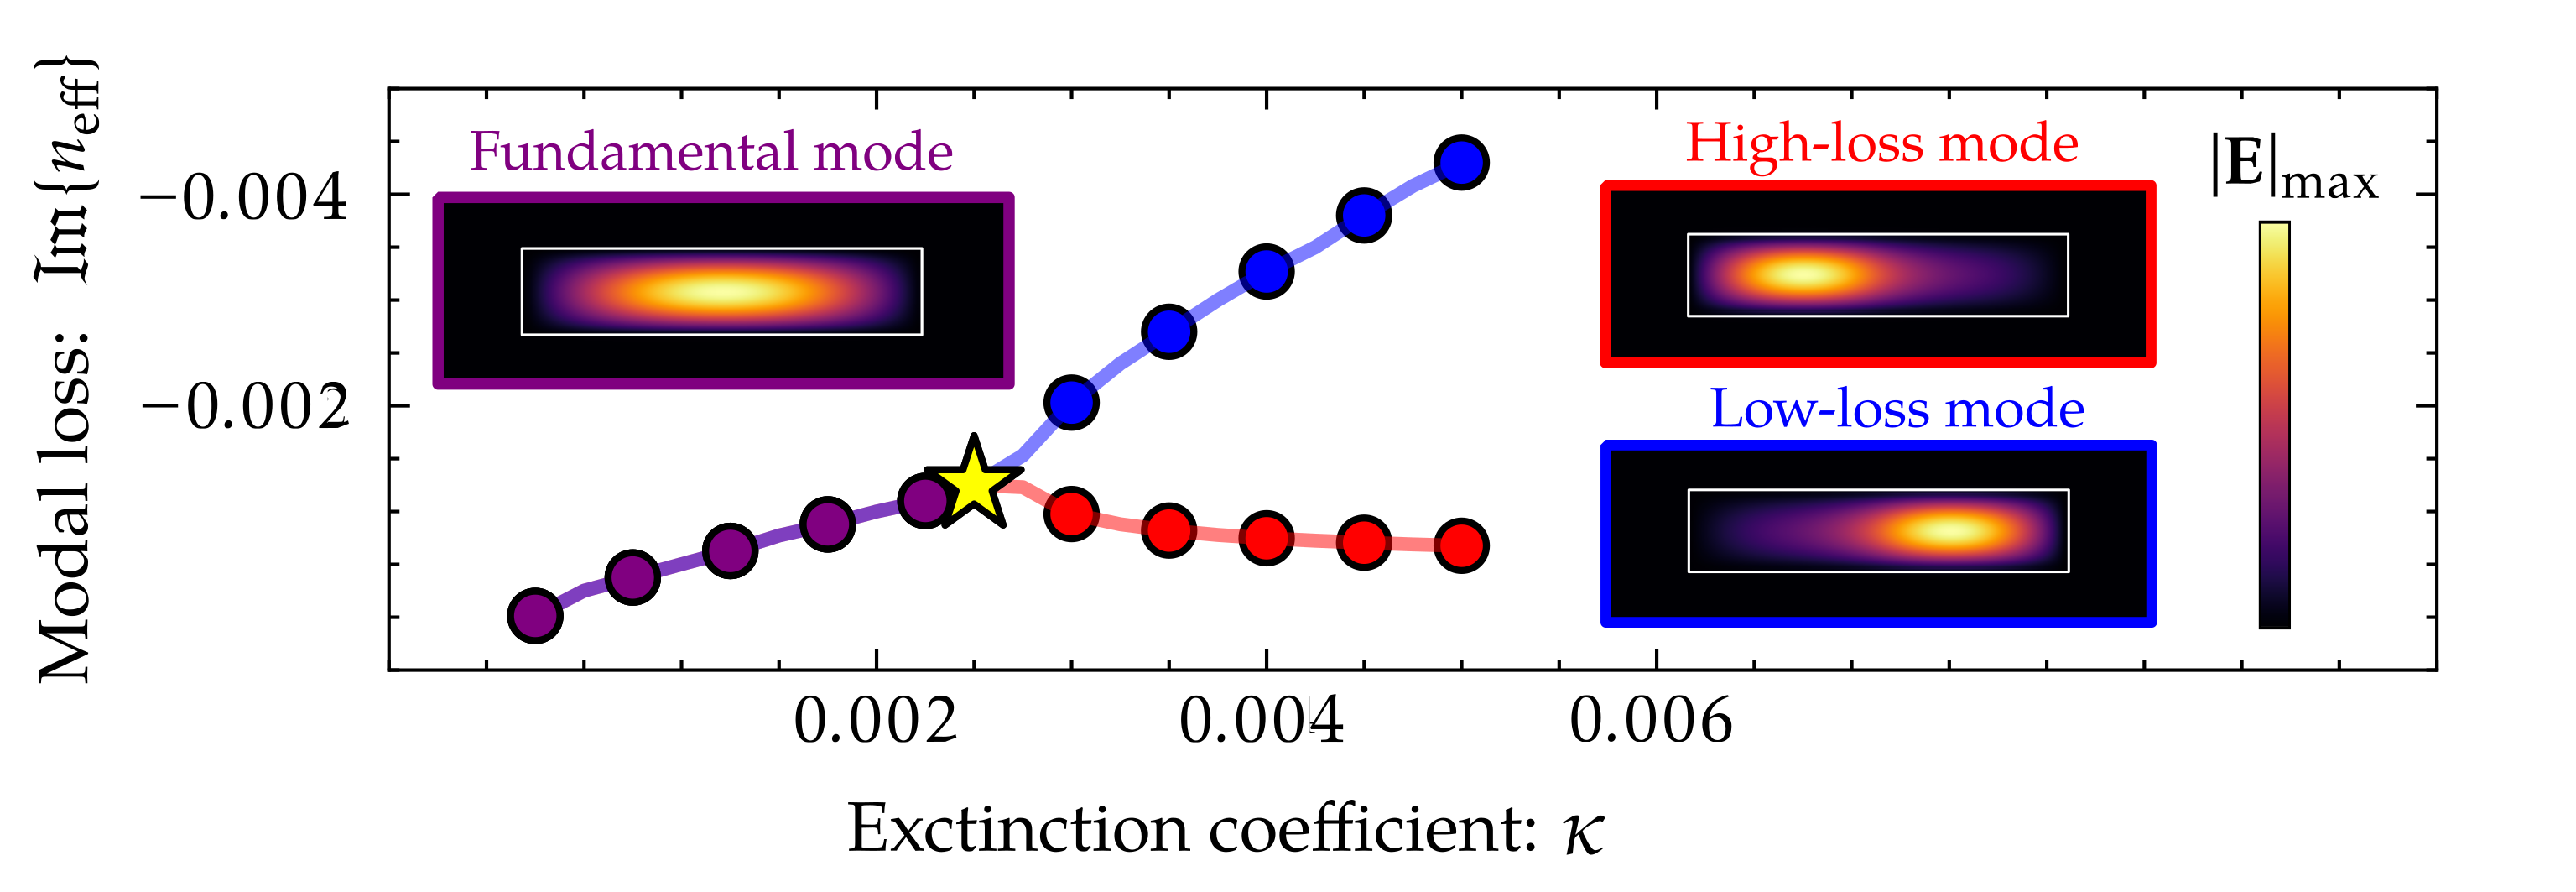
\includegraphics{figures/TOPS_pt.png}}%%
    \caption{Parity-time symmetry breaking and interpretation of losses of propagating modes. Make this figure look better.}
    \label{fig:thermo_opt}
\end{figure}

\subsection*{Topology optimization results~\cite{ownpub0}}

Inspired by PT-symmetry breaking waveguides, in~\cite{ownpub0} we use topology optimization to have good heat conduction and low optical loss in thermo-optical phase shifters.
The optimization problem considers a waveguide cross-section with a metallic heater, and seeks to minimize optical loss in an optical waveguide for both heated and 
unheated configurations. Unlike the eigenvalue-based approach in~\cite{lipson}, in this work we evaluate losses by solving a linear system of equations where we excite the waveguide 
and calculate the excited mode's 
amplitude. As illustrated in \figref{fig:thermo_opt}, maximizing the mode amplitude, is equivalent minimizing the width of the effective 
index resonance, and thus the loss of the mode. Based on this insight, we formulate the optimization problem, where we design the metalic heater around the waveguide, by using a worst-case maximization 
of the electric-field intensity at two effective indices corresponding to heated and unheated 
waveguide configurations. To integrate the heat problem into the topology optimization framework we use a linear material interpolation 
for the conductivity and an interpolation for the heat source
\begin{equation}
    Q(\hat{\rho})=P_{\text{in}} \frac{\hat{\rho}^p}{L a_e \sum_j \hat{\rho}_j}\,,
\end{equation}
where $P_\text{in}$ is the input power in the heater, $p=3$ is a penalization factor, and $a_e$ is the area of the element. With these interpolations we can solve a design-dependent
heat problem which then is fed into the optical problem to calculate the amplitude of the unheated and heated modes. To solve the inverse design
problem we derive a coupled adjoint sensitivity analysis, as further detailed in~\cite{ownpub0}, enabling the use of gradient-based optimization. CHECK AND
MENTION IF THE OPTIMIZE DEVICES RELY ON THE PT-SYMMETRY BREAKING EFFECT. COMMENT ON IT.

Using this framework we find the results in \figref{fig:thermo_res}, where we depict the optimized waveguide cross-section with a metallic heater, which is able to homogeneously heat the waveguide core,
allowing the same low-loss mode to propagate in both the heated and unheated scenarios. Moreover, several extensions of the topology optimization problem are considered for varying volume constraints, optical power, and including fabrication constraints (e.g., minimum lengthscales, and layered 
litography processes). SAY HOW MucH IMPROVEMENT WE GOT!

\begin{figure}[tb]
    \centering
    \makebox[\textwidth][c]{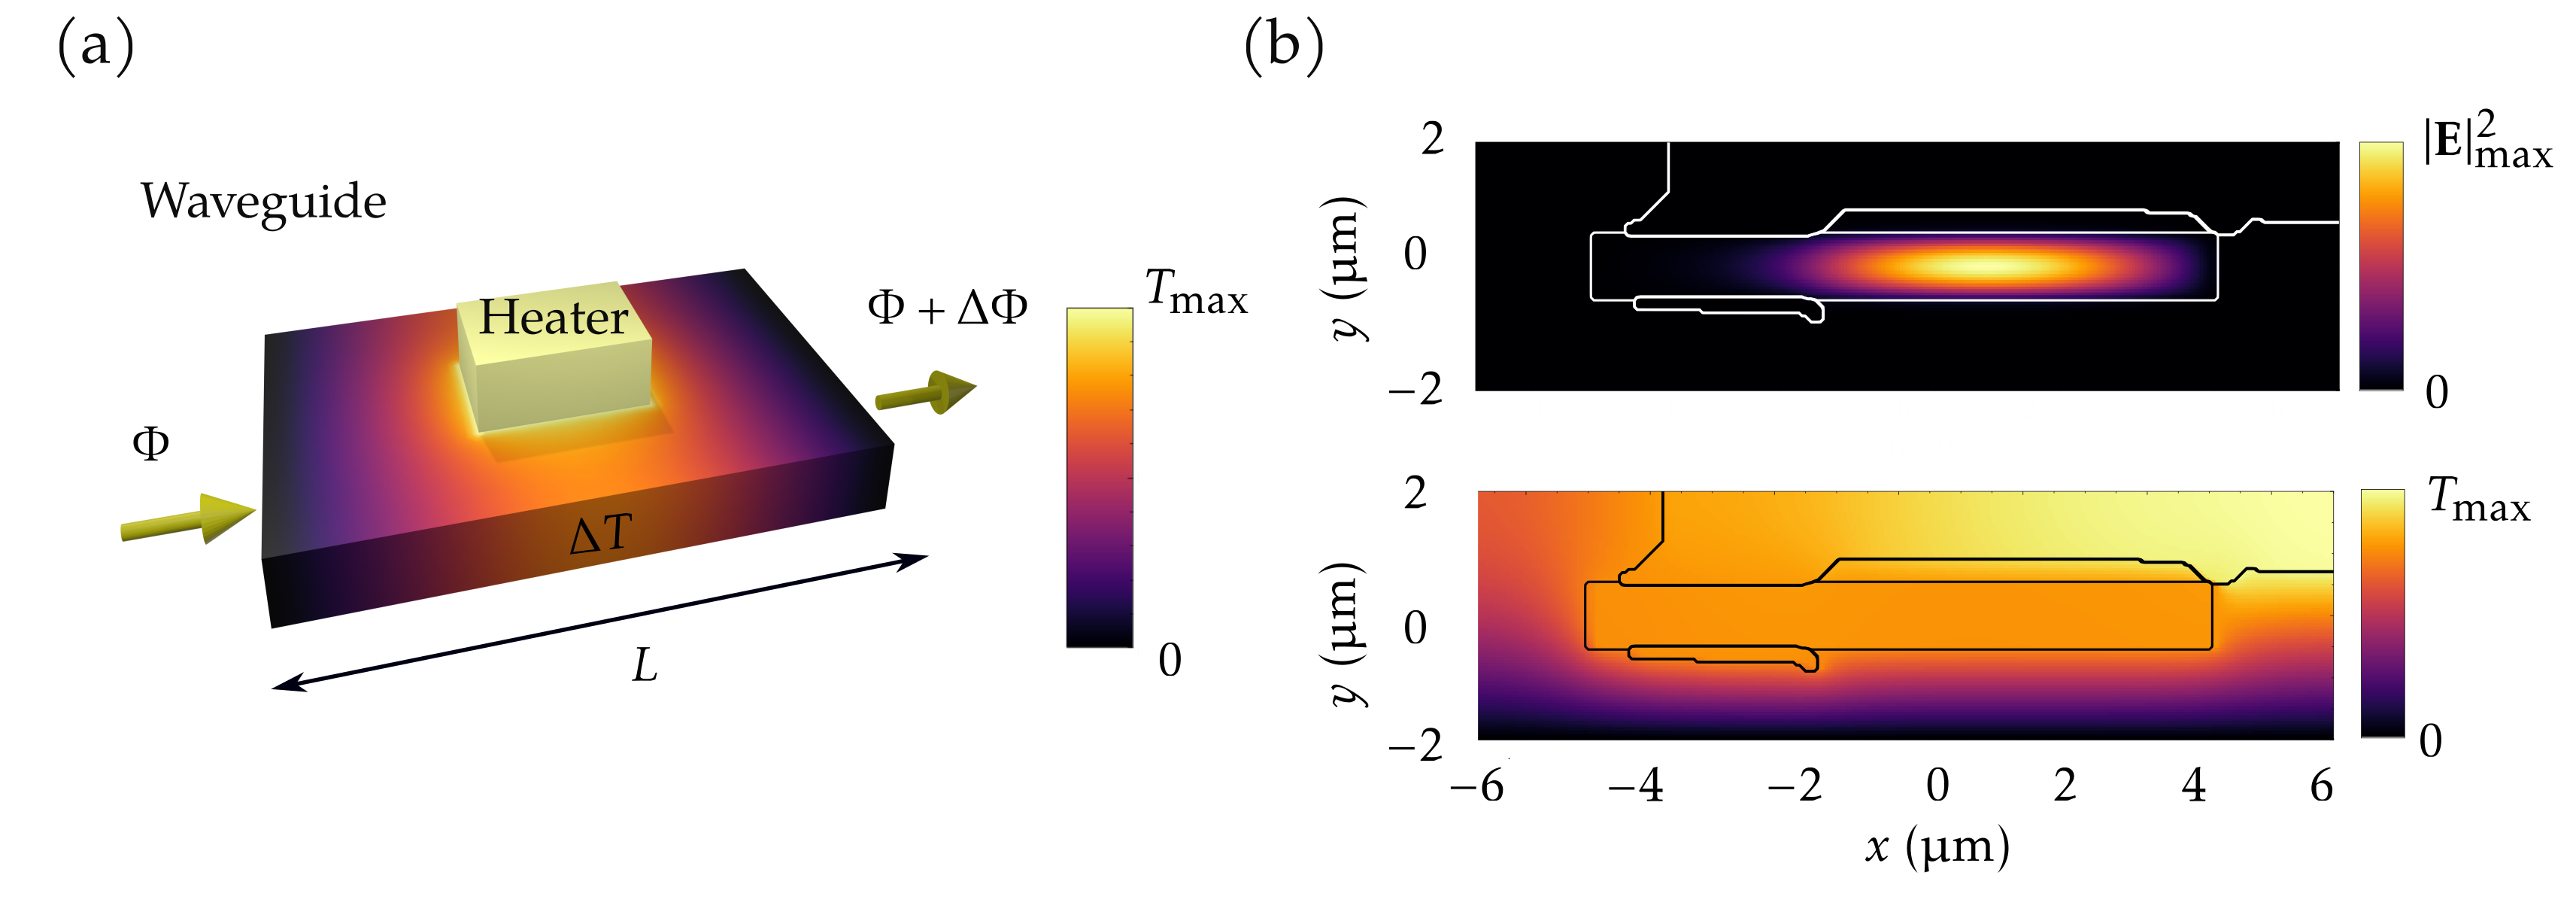
\includegraphics{figures/TOPS_results.png}}%%
    \caption{Topology optimization of thermo-optical phase-shifters. (a) Phase-shifting mechanism, where a heater changes the temperature in the waveguide $\Delta T$, which for a length $L$ creates a phase-shift
    $\Delta \Phi$. (b) Thermal and optical response of the topology optimized device. Adapted with permission from~\cite{ownpub0} \copyright Optical Society of America.}
    \label{fig:thermo_res}
\end{figure}

\subsection*{Outlook and future work}

The framework laid out in our work~\cite{ownpub0} opens up the avenue for the study and optimization to weakly coupled topology optimization problems. For example, for the design of phase-shifters and thermo-optical modulators, it should be straightforward to extend this
formalism to three dimensional system, where one could account for insertion/coupling losses of the integrated photonic circuits. Another example could be the to use multi-material topology optimization, to design not-only the heating
device, but also the optical waveguide. Finally, this formalism could be applied to design completely different devices, such as re-configurable photonic systems that might be modulated by an external heat source, or thermo-optical
switches based on optical cavities~\cite{switch, switch_2}, where the change in refractive index shifts the cavity in- or out-of-resonance.

SAY THAT CONDUCTION AND ELECTROSTATICS ARE SIMILAR CITE POCKELS PAPER AND TALK ABOUT ELECTRO-OPTICAL MODULATION!

\section{Towards strong coupling -- heat dissipation in optics}

In the strong coupling regime, the optical response will modify the thermal response, and vice versa.
For example, optical absorption can lead to significant local heating, altering the refractive index and modifying the optical field. 
This mutual dependence requires strongly a coupled treatment of the heat and optical problems, 
which can be accounted for by modeling the optical absorption with an electric field dependent volumetric heat source~\cite{plasm_heat_source}
\[
Q(\mathbf{r}) = \frac{1}{2} \omega \varepsilon_0 \operatorname{Im}[\varepsilon(\mathbf{r})] |\mathbf{E}(\mathbf{r})|^2,
\]
where the material losses ($\Im[\varepsilon]$) convert the electromagnetic energy into heat. 
This expression is particularly important in metal nanostructures, where plasmonic resonances can lead to localized temperature increases~\cite{plasm_heat_source}, or in 
high-intensity photonics where even low absorption materials can generate significant heat~\cite{thermal_nl, high_I_T}. Moreover, the thermo-optical feedback can give rise to nonlinear effects, such as self-focusing~\cite{thermal_nl}. As a matter of fact, if we still consider a linear
thermal response and thermo-optico coefficient,
the nonlinearity has the form of a Kerr-type nonlinearity ($\Delta n \propto \vert \mathbf{E} \vert^2$). Accouting and modeling
these effects could open up the avenue for the inverse design of novel nonlinear thermophotonic devices, with potential applications
in integrated nonlinear photonics~\cite{nl_photonics}, metasurfaces~\cite{nl_meta} and plasmonics~\cite{novotny}.


\section{Heat transfer as an auxiliary connectivity constraint}

Lastly, it is worthwile mentioning that the heat equation can be used as an auxiliary equation to enforce connectivity
and structural integrit in topology optimization problems~\cite{vanessa, structural_heat}, which is employed in several of our
works~\cite{ownpub1,ownpub2}. 

This method, introduced in~\cite{li_structural_2016}, is known as the Virtual Temperature
Method (VTM). The core idea of the VTM is to simulate a heat transfer problem on an auxiliary thermal field, where the design 
domain is treated as a heat source and a thermally conductive material, while void regions are modeled as an
insulating material, and a Dirichlet boundary condition ($T = 0$) is imposed on the boundaries where connectivity is required. When 
solving the steady-state heat equation [\eqref{eq:heat}], regions that are disconnected from the boundary 
cannot dissipate heat and therefore attain elevated temperatures. By applying a threshold criterion such as $T < T_\text{thresh}$, disconnected islands in the design can be 
detected and penalized. For instance, in our works~\cite{ownpub1,ownpub2} we compute a measure of the total virtual temperature
by integrating the temperature field over the design domain, and add it as a constraint in the optimization problem:
$\int_{\Omega_D} T \d \Omega \leq \epsilon_C$, where $\Omega_D$ is the design domain and $\epsilon_c$ is sufficiently small constant. This ensures that the final design remains physically connected to the required 
boundaries. 


Note that by appropriately selecting the connecting boundaries it is possible to use the VTM to enforce
structural integrity of the designs~\cite{structural_heat}, although this can also be ensured by solving an auxiliary
mechanical problem~\cite{structural_integrity}. For a more robust connectivity constraint formulation with less parameter tuning (e.g., material conductivies) we refer the reader to the Nonlinear 
Virtual Temperature Method (NVTM)~\cite{nvtm}, and for further details on connectivity constraints we refer the reader to the review 
article by Cool et al.~\cite{vanessa}.
